\documentclass[11pt]{article}
\usepackage[margin=1in]{geometry}
\usepackage{amsmath,amssymb,booktabs,graphicx,hyperref,xcolor,tikz}
\usepackage[capitalize,noabbrev]{cleveref}
\hypersetup{colorlinks=true,citecolor=blue,urlcolor=blue,linkcolor=blue}

\title{TRAIL-Hyper: Temporally Recurrent Reinforcement Learning for Multi-Resolution Semantic Abstraction of Evolving Knowledge Hypergraphs}
\author{Mohamed Bouchekouf(s)}
\date{}

\begin{document}
\maketitle

\begin{abstract}
Knowledge graphs extracted from scientific literature evolve through the arrival of entities, claims, datasets, and multi-way relations. Existing graph coarsening methods commonly reduce a pairwise graph, which can discard the arity and relation-level identity of knowledge-graph hyperedges. We formulate temporal semantic abstraction as the construction of a sequence of laminar hierarchies over cumulative knowledge-hypergraph snapshots. We propose TRAIL-Hyper, a framework combining a native hypergraph encoder, recurrent temporal state, and a reinforcement-learning (RL) policy that selects from bounded, admissible coarsening actions. The framework preserves hyperedges during collapse, assigns persistent super-node identities, logs temporal events, and constrains labels to contemporaneous evidence. We provide a reproducible implementation and an evaluation protocol covering structural/semantic coherence, temporal stability, label faithfulness, and question-grounded retrieval. We report preliminary reproducibility results for the executed structural, recurrent, and RL warm-start runs, while clearly separating unexecuted task and labelling metrics.
\end{abstract}

\section{Introduction}
Scientific knowledge bases contain relations that are naturally multi-way: a method may be evaluated on a dataset with a metric, while an article asserts a claim about several entities. Pairwise clique expansion turns a hyperedge of arity $n$ into $\binom{n}{2}$ edges and loses its single relation-level identity, arity, and endpoint multiplicity. This matters when abstractions must remain interpretable and useful for evidence-grounded research questions.

We study multi-resolution semantic abstraction of an evolving knowledge hypergraph. The output at every time is a laminar hierarchy, and across time it maintains stable super-node identities and a record of birth, growth, merge, split, and death events. RL has been used for graph coarsening \cite{taghibakhshi2021}, and recurrent encoders are established temporal modeling components. Our claim is not that either ingredient is new. Instead, the proposed contribution is an explicit formulation that joins higher-order hypergraph preservation, semantic--structural reconciliation, temporally informed sequential coarsening, laminarity, and evidence-faithful labels.

\section{Problem statement}
Let $\mathcal H_t=(V_t,E_t,X_t)$ denote a cumulative hypergraph at snapshot $t$, where $V_t$ is the node set, $E_t$ is a set of typed hyperedges, and $X_t$ stores node type, surface form, provenance, and time metadata. For a cutoff $\tau_t$, a node is included only if its \texttt{first\_seen\_year} is at most $\tau_t$, and a hyperedge is included only if its own year is at most $\tau_t$. This rule avoids future leakage.

The method returns partitions $\mathcal P_t^{(0)},\ldots,\mathcal P_t^{(L)}$. We require:
\begin{align}
&\mathcal P_t^{(0)}=\{\{v\}:v\in V_t\}, \\[-2mm]
&\forall C\in\mathcal P_t^{(\ell)},\ \exists! D\in\mathcal P_t^{(\ell+1)}\text{ such that }C\subseteq D, \label{eq:laminar}\\
&\bigcup_{C\in\mathcal P_t^{(\ell)}}C=V_t,\qquad C\cap C'=\varnothing\ (C\ne C'). \label{eq:partition}
\end{align}
Equations \ref{eq:laminar}--\ref{eq:partition} give nesting and non-overlap at every snapshot. A persistent identifier map matches clusters in $\mathcal P_{t-1}^{(L)}$ and $\mathcal P_t^{(L)}$ using member overlap and semantic compatibility without accessing $t+1$.

\section{Method}
\subsection{Native hypergraph and semantic encoding}
We use the incidence structure directly. A hypergraph encoder produces $z_{v,t}$ for each node from typed hyperedge incidence, relation type, node type, and semantic features derived from contemporaneous \texttt{surface\_form} fields. A recurrent state then summarizes temporal context:
\begin{equation}
h_{v,t}=\operatorname{GRU}(z_{v,t},h_{\pi(v),t-1}),
\end{equation}
where $\pi$ identifies a persistent predecessor when available; a new node receives an initial state. The GRU is an architectural mechanism, not the main novelty.

\paragraph{Neo4j representation.} We store the hypergraph in Neo4j without a clique expansion. Each entity is an \texttt{:Entity} node; each hyperedge is a first-class \texttt{:Hyperedge} node; and directed \texttt{:HAS\_MEMBER} relationships carry endpoint position. Thus an arity-$n$ relation remains one Neo4j node with $n$ incidence relationships. A temporal Cypher query filters both hyperedge year and entity first-seen year. This storage model supports visual inspection while the coarsening algorithm retains native incidence.

\subsection{Bounded RL coarsening}
At level $\ell$, the state contains current clusters, their embeddings, coarse hyperedges, and recurrent summaries. A deterministic hypergraph-aware routine generates a bounded candidate set
\begin{equation}
\mathcal A_t^{(\ell)}=\{(C_i,C_j):\operatorname{compatibility}(C_i,C_j)>0\}.
\end{equation}
The policy chooses an admissible merge, rather than an arbitrary node pair, avoiding an $O(|V|^2)$ action space. The repository includes a small REINFORCE policy over structural/semantic action features as a reproducible starter; a HyperGNN--PPO policy is a planned replacement behind the same interface.

For a candidate merge, the reward is
\begin{equation}
R=\lambda_sR_{\mathrm{struct}}+\lambda_mR_{\mathrm{sem}}+\lambda_tR_{\mathrm{temp}}+\lambda_hR_{\mathrm{hier}}-\lambda_cR_{\mathrm{complexity}}.
\label{eq:reward}
\end{equation}
Here $R_{\mathrm{struct}}$ rewards keeping endpoints of native hyperedges together, $R_{\mathrm{sem}}$ rewards semantic agreement, and $R_{\mathrm{temp}}$ rewards justified continuity. $R_{\mathrm{hier}}$ is a hard-by-construction constraint: actions merge only existing clusters, guaranteeing \cref{eq:laminar}. Complexity penalties prevent a single giant cluster or uninformative singleton parents. This design makes the semantic--structural trade-off explicit instead of defaulting to text-only or topology-only clustering.

\subsection{Hyperedge collapse}
For $e=(v_1,\ldots,v_n)$ and parent map $c$, we map each endpoint to $c(v_i)$ and retain a typed, weighted coarse hyperedge:
\begin{equation}
\bar e=(\operatorname{type}(e),\{c(v_i)\}_{i=1}^{n},\{\#\{i:c(v_i)=u\}\}_{u\in\bar e}).
\end{equation}
If all endpoints map to one super-node, $e$ becomes internal evidence rather than an inter-super-node edge. If only some coalesce, the surviving coarse hyperedge retains endpoint multiplicities. If three or more super-nodes remain, it is retained as a multi-way coarse hyperedge, never decomposed into pairs. This loses individual endpoint identity within a super-node, but preserves arity, relation type, and multiplicity.

\subsection{Temporal identity and labels}
We greedily match new clusters to old identities using Jaccard overlap above a threshold, with semantic similarity as an extension point. Unmatched clusters are births; unmatched prior identities are deaths; one-to-many and many-to-one overlaps define splits and merges. Temporal regularization improves continuity but can reduce the best single-snapshot partition; this cost is measured rather than hidden.

Labels are generated only from a logged prompt containing the snapshot cutoff, member surface forms, node-type counts, and internal evidence. The labeller is instructed to make no unsupported claim. Faithfulness is measured by the support rate of label terms in the evidence and an over-claim rate assessed against member facts. Earlier-snapshot labels may not mention later evidence.

\section{Experimental protocol}
The provided Collection 10 export contains 5,798 nodes and 1,429 hyperedges. We use at least three cumulative snapshots (e.g., 2022, 2024, and 2026) and report node/edge growth, node-type counts, relation counts, hyperedge-arity distributions, time span, and missing/invalid timestamps.

\begin{figure}[t]
\centering
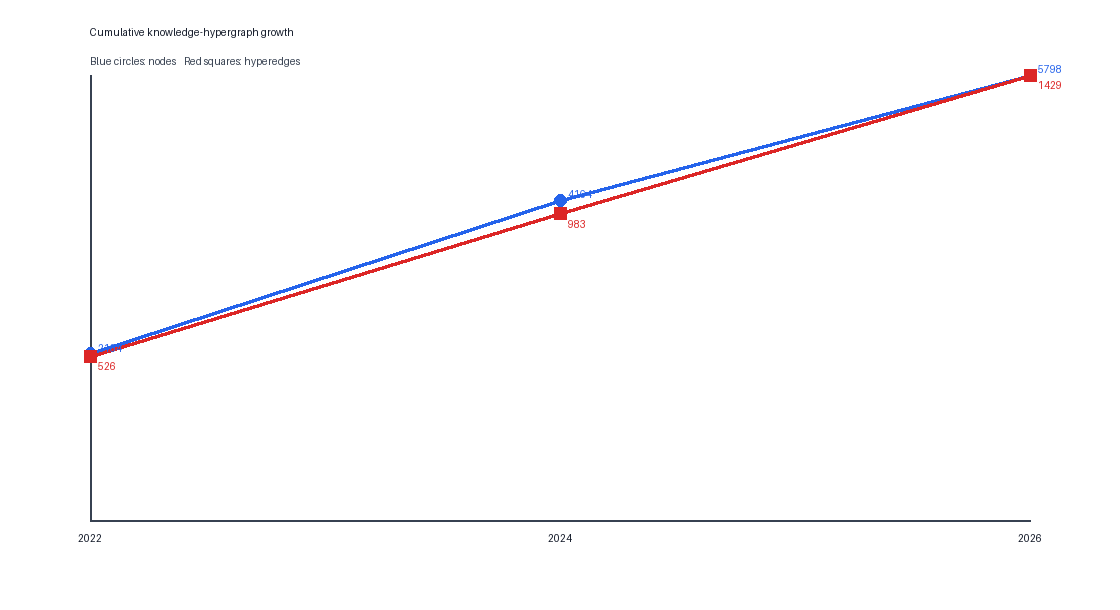
\includegraphics[width=.82\linewidth]{figures/snapshot_growth.png}
\caption{Cumulative knowledge-hypergraph growth. The snapshots contain 2,164/4,164/5,798 nodes and 526/983/1,429 native hyperedges.}
\label{fig:growth}
\end{figure}

\begin{figure}[t]
\centering
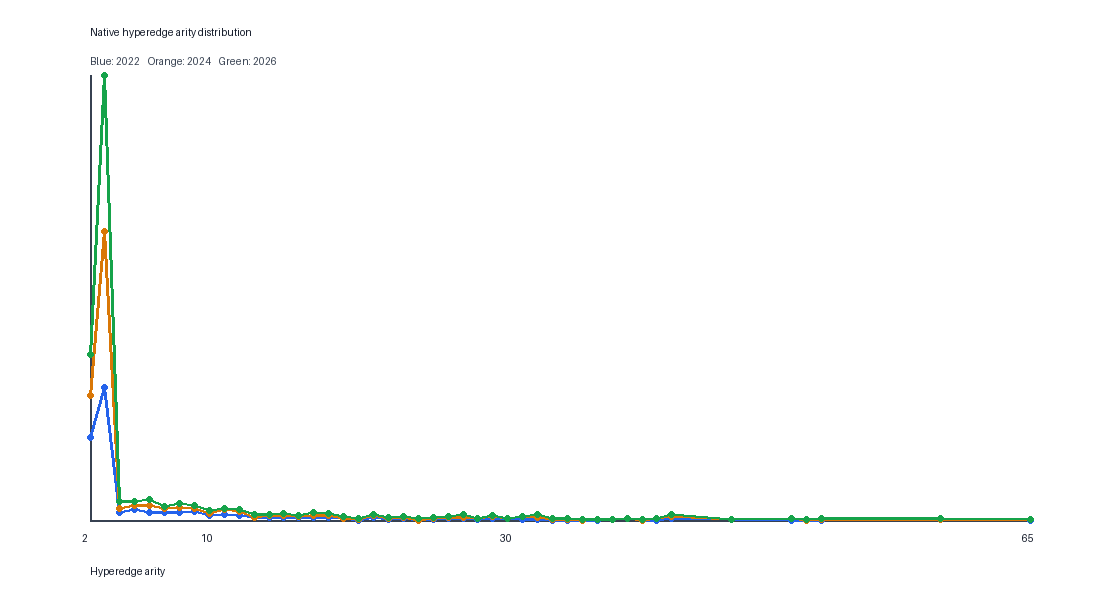
\includegraphics[width=.82\linewidth]{figures/arity_distribution.png}
\caption{Native hyperedge-arity distributions. The long tail motivates hypergraph-native processing: clique projection would introduce 20,760, 47,983, and 72,701 pairwise edges at the three cutoffs.}
\label{fig:arity}
\end{figure}

\paragraph{Baselines.} We compare (i) native deterministic coarsening without RL or recurrent state, (ii) clique expansion followed by pairwise graph clustering, (iii) semantic-only clustering, (iv) native coarsening without temporal state, and (v) the full model. Ablations isolate structural, semantic, and temporal reward terms.

\begin{figure}[t]
\centering
\begin{tikzpicture}[node distance=6mm and 5mm, every node/.style={draw,rounded corners,align=center,font=\small}, >=latex]
\node (h) {Temporal\\hypergraph};
\node (e) [right=of h] {Native encoder\\+ semantics};
\node (g) [right=of e] {GRU temporal\\state};
\node (p) [right=of g] {Bounded RL\\merge policy};
\node (l) [below=of p] {Laminar hierarchy\\+ coarse hypergraph};
\node (o) [left=of l] {Persistent IDs,\\events, labels};
\draw[->] (h)--(e); \draw[->] (e)--(g); \draw[->] (g)--(p); \draw[->] (p)--(l); \draw[->] (l)--(o);
\end{tikzpicture}
\caption{TRAIL-Hyper architecture. Native hypergraph structure and semantic signal inform temporally conditioned, bounded coarsening actions.}
\label{fig:architecture}
\end{figure}

\paragraph{Metrics.} Coherence includes native hyperedge retention and within-cluster semantic similarity. Temporal stability includes aligned membership agreement, identity survival, and event rates. Label quality includes support rate and over-claim rate. The extrinsic evaluation uses the question/ground-truth set: retrieve method-containing super-nodes for each question and compute Recall@$k$, MRR, and citation-evidence coverage. Pairwise projection loss is quantified by the number of induced pairwise edges, loss of native hyperedge identity/multiplicity, and change in downstream retrieval.

\subsection{Preliminary reproducibility results}
We executed the registered one-level protocol on cumulative 2022, 2024, and 2026 snapshots. ``Retention'' is the mean native-hyperedge retention across the three snapshots; ``stability'' is the mean membership agreement across the two adjacent snapshot pairs. The semantic--structural row uses the seeded GRU temporal state. The RL result is a seeded, single 2022-snapshot REINFORCE run in which the policy controls the first 128 admissible merges; it is not a claim of converged policy performance. These results establish that the pipeline runs end-to-end and expose the expected retention--stability trade-off: semantic emphasis improves temporal agreement but reduces structural retention.

\begin{figure}[t]
\centering
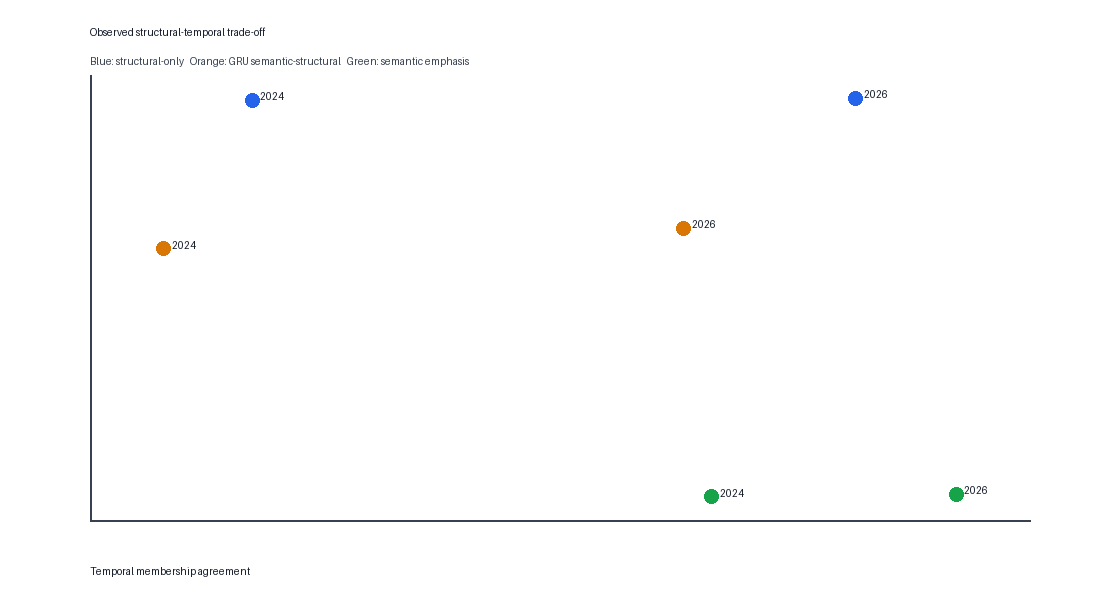
\includegraphics[width=.82\linewidth]{figures/retention_stability.png}
\caption{Observed trade-off among executed baselines. Each point is a transition endpoint (2024 or 2026); higher and further right is preferable.}
\label{fig:tradeoff}
\end{figure}

\begin{table}[t]
\centering
\caption{Observed preliminary results. Dashes denote metrics not yet executed, not zero scores.}
\label{tab:preliminary}
\begin{tabular}{lrrrr}
\toprule
Method & Snapshots & Retention $\uparrow$ & Stability $\uparrow$ & Clusters\\
\midrule
Structural-only native & 2022--2026 & 0.9229 & 0.9134 & 1082/2082/2899\\
GRU semantic--structural & 2022--2026 & 0.8621 & 0.8958 & 1082/2082/2899\\
Semantic-emphasis native & 2022--2026 & 0.7579 & 0.9515 & 1082/2082/2899\\
GRU + REINFORCE warm start & 2022 & 0.8511 & -- & 1082\\
\bottomrule
\end{tabular}
\end{table}

The question-grounded retrieval metrics (Recall@$k$ and MRR), the pairwise clique-projection baseline, and label support/over-claim scores are deliberately not included in \cref{tab:preliminary}, because they require an explicit retrieval and labelling run over \texttt{questions.csv} and \texttt{ground\_truth.json}. They are registered evaluation components, not completed results.

\section{Reproducibility and limitations}
The code fixes snapshot construction, preserves data provenance, writes event logs, exports DOT diagrams, stores native incidence in Neo4j, and exposes the exact labeller input. It includes a seeded GRU temporal baseline and a seeded REINFORCE bounded-action policy; it should not be described as a completed, fully trained HyperGNN--PPO system. RL training can be sample-inefficient on a corpus with only 52 source articles; candidate pruning, warm starts from deterministic coarsening, held-out temporal cutoffs, and comparison to simple baselines are therefore essential. Further, automated labels can summarize evidence but cannot establish truth beyond the extracted corpus.

\section{Conclusion}
TRAIL-Hyper formulates interpretable abstraction of evolving knowledge hypergraphs as a native, temporal, sequential coarsening problem. Its main testable hypothesis is that temporal state and learned bounded merge decisions improve stability and task-grounded retrieval without sacrificing higher-order structure or label faithfulness.

\bibliographystyle{plain}
\bibliography{references}
\end{document}
